\documentclass[a4paper]{article}
\usepackage[utf8]{inputenc}
\usepackage{authblk}
\usepackage[misc]{ifsym}
\usepackage{geometry}
\usepackage{graphicx}
\usepackage{subfigure}
\usepackage{pifont}
\usepackage{array}
\usepackage{booktabs}
\usepackage{float}
\usepackage{multirow}
\usepackage{multicol}
\usepackage[sorting=none]{biblatex}
\addbibresource{ref.bib}
\geometry{left=2cm, right=2cm, top=2.0cm, bottom=2.0cm}
% Put all your figures in this folder
\graphicspath{{./Figures/}}

\title{Title}
\author[a]{Author1}

\affil[a]{School of Sexy Tea, Sexy Tea University \authorcr author1@mail.Sexy Tea.edu.cn}
\date{7 Oct 1997}

\begin{document}

\maketitle
\begin{abstract}
    \noindent This is your abstract. This is your abstract. This is your abstract. This is your abstract.
    \newline
    \newline
    \emph{Keywords: keywords1; keywords2; keywords3; keywords4}
    
\end{abstract}

\section{Introduction}
This is introduction part.
\newline
\newline
The template of citations: \cite{ref1}
\newline
\newline
The template of figures
\begin{figure}[H]
    \centering
    \subfigure[]{
    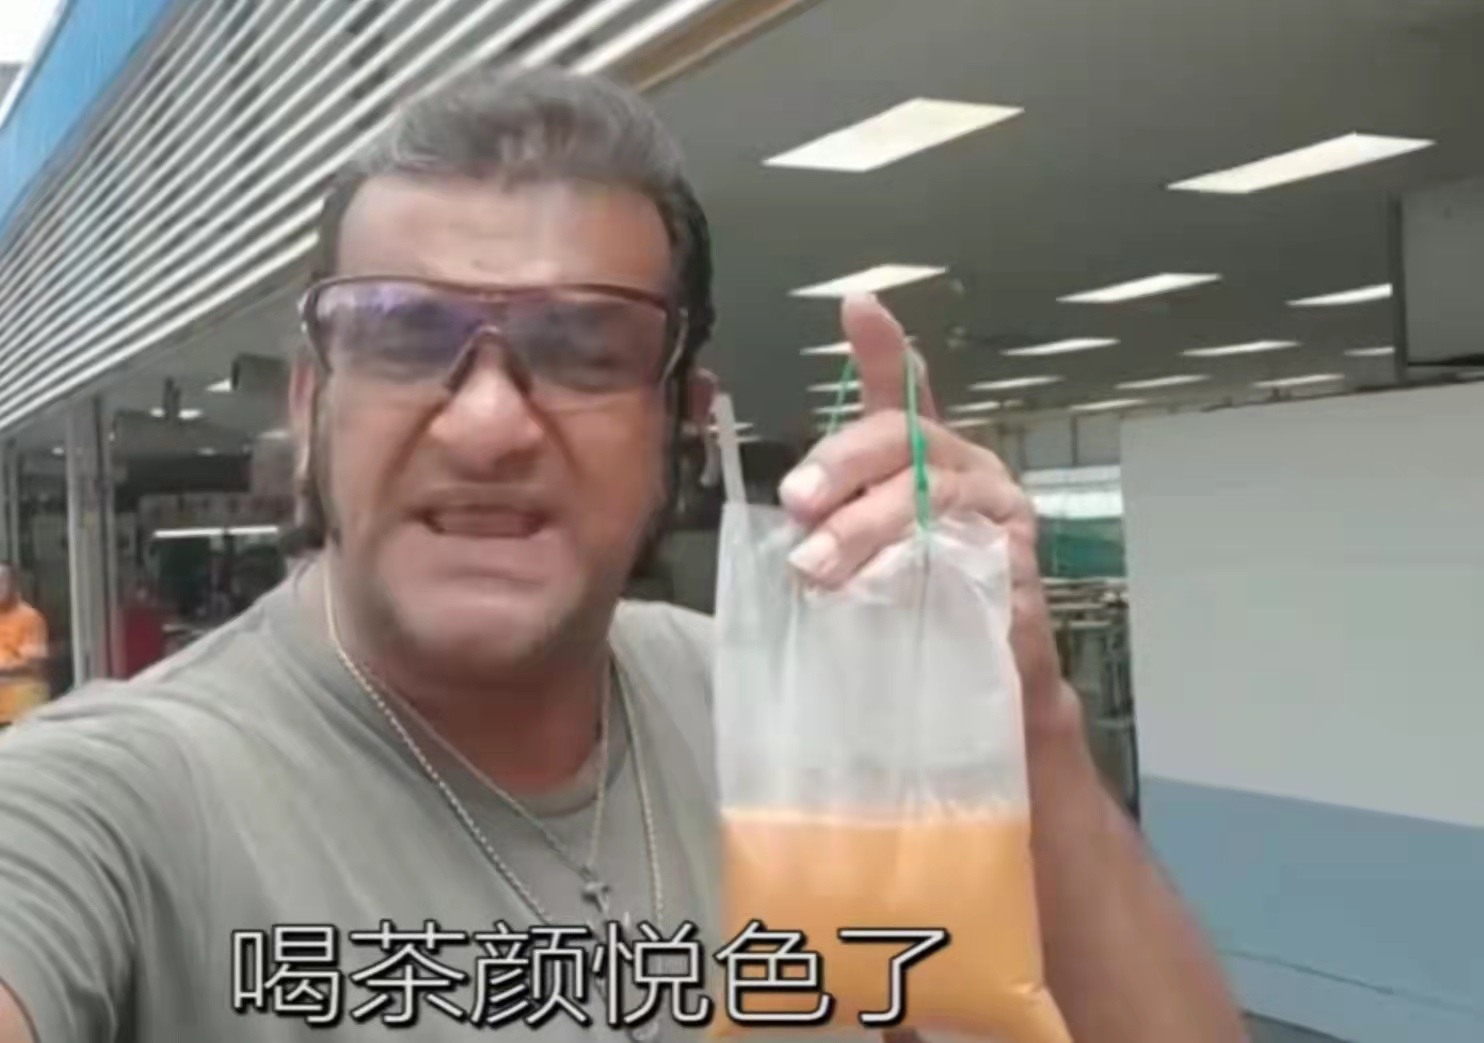
\includegraphics[scale=0.1]{1}}
    \subfigure[]{
    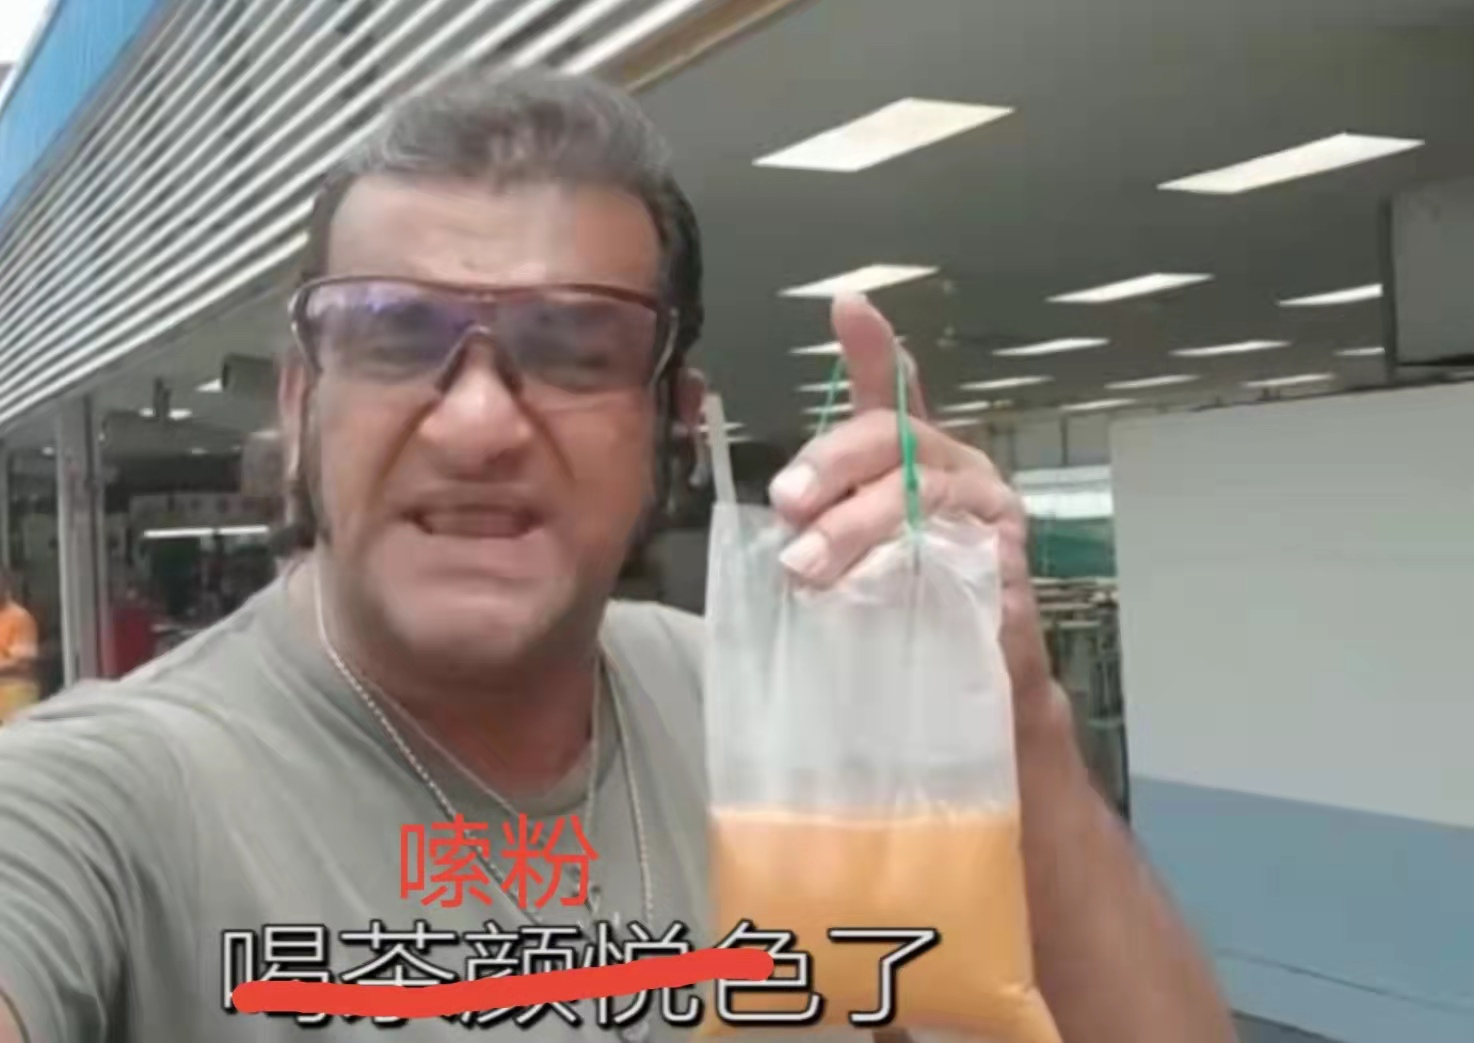
\includegraphics[scale=0.1]{2}}
    \caption{Drink Sexy Tea!. (a)Drink Sexy Tea!. (b)Drink Sexy Tea!.}
    \label{fig:1}
\end{figure}

\section{Related works}
\subsection{Subsection1}
This is subsection1.

\subsection{Subsection2}
This is subsection2.

\section{Method}
This is method part.

\section{Experiments}
This is experiment part.

\subsection{Results and discussions}
This is results and discussions.
\newline
\newline
The template of tables:
\begin{table}[H]
    \centering
    \begin{tabular}{ccc}
        \hline
        \specialrule{0em}{1pt}{1pt}
        \multirow{2}{*}{Ground-truth} & \multicolumn{2}{c}{Prediction} \\
        \cline{2-3}
        & Positive & Negative \\
        \hline
        \specialrule{0em}{1pt}{1pt}
        Positive & TP & FN\\
        \specialrule{0em}{1pt}{1pt}
        Negative & FP & TN\\ 
        \hline
    \end{tabular}
    \caption{Confusion matrix}
    \label{tab:my_label}
\end{table}

\noindent Another template of tables
\begin{table}[H]
    \centering
    \begin{tabular}{ccccc}
    \hline
    \specialrule{0em}{1pt}{1pt}
    Sexy Tea & Sexy Tea & Sexy Tea & Sexy Tea & Sexy Tea \\
    \hline
    \specialrule{0em}{1pt}{1pt}
    Sexy Tea & Sexy Tea & 100\% & 100 MB & 100 \\
    \specialrule{0em}{1pt}{1pt}
     & Sexy Tea & 100\% & 100 MB & 100 \\
    \specialrule{0em}{1pt}{1pt}
    Sexy Tea & Sexy Tea & 100\% & 100 MB & 100 \\
    \specialrule{0em}{1pt}{1pt}
    Sexy Tea & Sexy Tea & 100\% & 100 MB & 100 \\
    \hline
    \end{tabular}
    \caption{Comparison of Sexy Tea}
    \label{tab:2}
\end{table}

\noindent The template of ablation study
\begin{table}[H]
    \centering
    \begin{tabular}{ccccccc}
    \hline
    \specialrule{0em}{1pt}{1pt}
    Sexy Tea & Sexy Tea & Sexy Tea & Sexy Tea & Sexy Tea & Sexy Tea & Sexy Tea \\
    \hline
    \specialrule{0em}{1pt}{1pt}
    \ding{51} & & & & 100\% & 100 MB & 100 \\
    \specialrule{0em}{1pt}{1pt}
     & \ding{51} & & & 100\% & 100MB & 100\\
    \specialrule{0em}{1pt}{1pt}
    & \ding{51} & \ding{51} & & 100\% & 100 MB & 100 \\
    \specialrule{0em}{1pt}{1pt}
    & \ding{51} & \ding{51} & \ding{51} & 100\% & 100 MB & 100\\
    \hline
    \end{tabular}
    \caption{Ablation studies for 100.}
    \label{tab:3}
\end{table}

The template of equations:
\begin{equation}
    Precision=\frac{TP}{TP+FP}
\end{equation}

\begin{equation}
    Recall=\frac{TP}{TP+FN}
\end{equation}

\section{Conclusions}
This is conclusion part.
\par1. Conclusion 1.
\par2. Conclusion 2.
\par3. Conclusion 3.

\printbibliography

\end{document}
